\chapter{RSA攻击}

\section{实验目的}

本次实验的目的是探索 RSA 在不正确生成模 $N$ 的情况下的安全性。

\section{实验要求}

在 RSA 的密钥生成阶段,不同用户应该独立的生成模 $N$,即选取大素数 $p$ 和 $q$
相乘得到 $N$。假设某个项目中的 RSA 具体实现过程如下:1)首先随机选取一
个随机数 $R$ 然后选取距离 $R$ 最近的素数 $p$,以及另外一个相近的素数 $q$。2)$p$
和 $q$ 相乘得到 $N$。由于 $p$ 和 $q$ 为相近的两个素数,在此情况下存在对 $N$ 的高效
分解方法,导致方案不安全。

假设$N$的因子$p$和$q$满足:
\begin{equation}
    \label{eq:pq}
    |p-q|<2N^{1/4}
\end{equation}

那么$N$的分解可由如下分析得出:

令$A=(p+q)/2$,那么根据式\ref{eq:pq},能够得到$A-\sqrt{N}<1$。
因此可以根据$A=\left\lceil \sqrt{N}\right\rceil $计算得到$A$。

下图展示了$p,q,\sqrt{N},(p+q)/2$之间的关系。

\begin{figure}[!htbp]
    \centering
    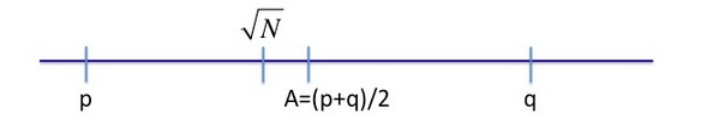
\includegraphics[width=0.8\textwidth]{figures/RSA.png}
\end{figure}

由于$N=pq=(A-x)(A+x)=A^2-x^2$,因此有$x=\sqrt{A^2 - N}$。当求得
$x$以后,容易根据$p=A+x,q=A-x$得到$N$的分解。

根据上述分析,请完成挑战(在实验内容中给出)。

\section{实验内容}

\subsection{分解挑战1}

如下的整数$N$是两个素数$p,q$的乘积,且满足$|p-q|<2N^{1/4}$,请分解
整数N并给出其十进制结果。\\

$
\begin{aligned}
    N = &17976931348623159077293051907890247336179769789423065727343008115 \\
        & 77326758055056206869853794492129829595855013875371640157101398586 \\
        & 47833778606925583497541085196591615128057575940752635007475935288 \\
        & 71082364994994077189561705436114947486504671101510156394068052754 \\
        & 0071584560878577663743040086340742855278549092581
\end{aligned}
$\\

本次实验采用了Python语言编写脚本,并利用了gmpy2库进行大整数的高精度运算。

挑战1的求解代码如下:
\begin{lstlisting}[language = Python]
def factoring_1(N):
    A, r = gmpy2.isqrt_rem(N)   ## 求平方根
    if r > 0:
        A += 1
    A_squared_minus_N = A**2 - N
    x = gmpy2.isqrt(A_squared_minus_N)
    p = A - x
    q = A + x
    N_slash = gmpy2.mul(p, q)
    assert N == N_slash         ## 检查N是否分解成功
    return p, q
\end{lstlisting}

该部分攻击原理实验要求中已经给出,因此不再赘述。

需注意,此处传入的$N$为一个大整数,因此需要使用gmpy2库中的mpz方法初始化。此外,后续的开方,乘法
操作,都需要使用gmpy2库中的各方法进行,否则会引起错误。

最终得到:

$
\begin{aligned}
    p = &134078079299425970995740249982058461274793658205923933777235614437\\
        &217640300736627688911116143623269986750405460943393208384195233759\\
        &86027530441562135724301\\
    q = &134078079299425970995740249982058461274793658205923933777235614437\\
        &217640300737785609803489305577505696600492340021925908230851639400\\
        &25485114449475265364281
\end{aligned}
$\\

\subsection{分解挑战2}

如下的整数$N$是两个素数$p,q$的乘积,且满足$|p-q|<2^{11}N^{1/4}$,请分解
整数N并给出其十进制结果。\\

$
\begin{aligned}
    N = &6484558428080716696628242653467722787263437207069762630604390703787\\
        & 9730861808111646271401527606141756919558732184025452065542490671989 \\
        & 2428844841839353281972988531310511738648965962582821502504990264452 \\
        & 1008852816733037111422964210278402893076574586452336833570778346897 \\
        & 15838646088239640236866252211790085787877
\end{aligned}
$\\

挑战2的求解代码如下:
\begin{lstlisting}[language = Python]
def factoring_2(N):
    N_sqrt, r = gmpy2.isqrt_rem(N)
    if r > 0:
        N_sqrt += 1
    for offset in range(2**20):
        A = N_sqrt + offset
        A_squared_minus_N = A**2 - N
        x = gmpy2.isqrt(A_squared_minus_N)
        p = A - x
        q = A + x
        if gmpy2.mul(p, q) == N:
            break
    return p, q
\end{lstlisting}

此处与挑战1的不同是,$|p-q|$增大了,但仍有$A-\sqrt{N}< 2^20$,可从$\sqrt{N}$开始搜索$A$的值。

我们枚举偏移量$offset \in \left[0, 2^{20}\right)$,尝试利用$p=A+x=A+\sqrt{A^2-N}$对$N$进行分解,
当分解成功时返回$p,q$。

最终得到:

$
\begin{aligned}
    p = &254647961469961834380088165639739422293414542685241578463285819278\\
        &857779699852228351438510732495734541073844615571931733044972448140\\
        &71505790566593206419759\\
    q = &254647961469961834380088165639739422293414542685241578463285819278\\
        &857779701063980544912465269708141676325635095417847347418713798566\\
        &82354747718346471375403
\end{aligned}
$\\

\subsection{解密挑战}

如下所示是使用分解挑战 1 中的模数 N 对一段消息进行加密得到的密文。其中
加密指数 e=65537。明文消息使用 ASCII 进行编码后使用 PKCS v1.5 进行消
息填充,需要指出的是,消息中使用'0x00'对消息和随机填充进行分割,而不
是'0xFF'。请在实验报告中给出下列密文的解密结果。\\

$
\begin{aligned}
    &220964518674103817763065611348834180174100697878928310717318391436761\\
        &356001205380042823296504735094243439462197515122564658399679428894607\\
        &645420405815647489880137348641204523252293201764879166664029975091887\\
        &299716905260832220677716000193292608700095799937240774589677736978175\\
        &71267229951148662959627934791540
\end{aligned}
$\\

由于挑战1中已经对模数$N$进行了分解得到了$p,q$,因此后续进行解密是较为简单的。
具体步骤如下:
\begin{enumerate}
    \item 计算$\varphi(N) = (p-1)(q-1)$;
    \item 计算私钥$d = e^{-1} \bmod \varphi(N)$;
    \item 利用解密公式获得明文消息:$m = c^d \bmod N$。
    \item 找到分割字符'0x00',将明文消息分割为随机填充和消息,获得最后结果。
\end{enumerate}

求解代码如下:
\begin{lstlisting}[language = Python]
def decrypt(c, e, n):
    p, q = factoring_1(n)
    phi_n = gmpy2.mul(p - 1, q - 1)
    d = gmpy2.invert(e, phi_n)
    msg_hex = hex(gmpy2.powmod(c, d, n))[2:]

    ## PKCS v1.5 '0x02'开头,需补位
    if msg_hex[0] == '2':
        msg_hex = '0' + msg_hex
    
    ## 消息分割,取消息,去随机填充
    msg = msg_hex.split('00')[1]

    return str(bytes.fromhex(msg))
\end{lstlisting}

最后得到的消息为:
\begin{center}
    Factoring lets us break RSA.
\end{center}